\chapter{Simulazione}
Data la straordinarietà degli eventi che erano in corso dal punto di vista sanitario nel nostro paese si è reso necessario svolgere gran parte del lavoro in modalità a distanza e quindi senza la possibilità di testare il modello matematico appena ottenuto e i successivi risultati dovuti all'azione di controllo sul V.A.B. Il lavoro quindi è stato svolto per la maggior parte sfruttando il tool \textit{Simulink} di Matlab che è, in poche parole, un risolutore di equazioni differenziali.

Abbiamo così adottato una metodologia di lavoro basata su prototipi sempre più simili a quello che dovrebbe essere il sistema reale.
\section{Simulazione del sistema reale}
Il primo compito che abbiamo risolto è stato quello di implementare le equazioni differenziali ottenute nel capitolo precedente:
\begin{itemize}
	\item $\ddot{\phi} = f_{\ddot{\phi}} (M_c,\theta,\dot{\theta},C_m)$
	\item $\ddot{\theta} = f_{\ddot{\theta}} (M_c,\theta,\dot{\theta},C_m)$
\end{itemize}

Dove $M_c$ sarebbe la massa del passeggero, $\theta e \dot{\theta}$ lo stato del sistema e $C_m$  la coppia erogata dal motore. Si può notare come entrambe le equazioni differenziali siano indipendenti dalla coordinata libera $\phi$.
 \begin{figure}[H]
	\centering   	
	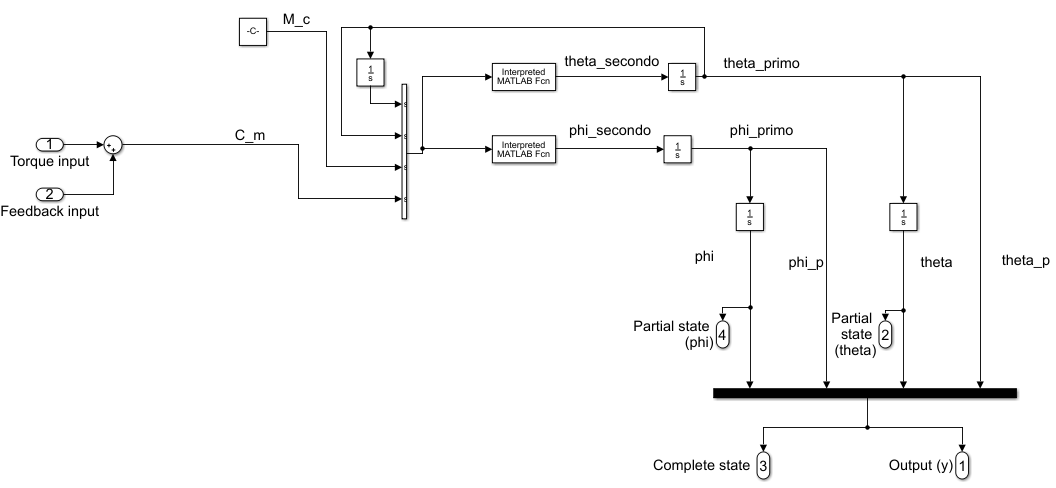
\includegraphics[width=1\textwidth]{Immagini/non_linear_system.png}
	\caption{Implementazione simulink delle equazioni differenziali}
	\label{fig:non_linear_system}
\end{figure}
In Fig.\ref{fig:non_linear_system} le \textit{interpreted function} altro non sono che  $f_{\ddot{\phi}}$ e $f_{\ddot{\theta}}$. A valle di esse sono presenti degli integratori che permettono di ottenere lo stato $x$ completo del sistema. Si può facilmente notare come $\dot{\theta} e \theta$ siano collegate direttamente all'input delle \textit{interpreted function}.
Si è dunque proceduto a  simulare il sistema per verificare la bontà di quanto ottenuto; in particolare, il sistema in anello aperto, dovrebbe oscillare all'infinito vista la mancanza di attriti nel modello.

\begin{figure}[H]
	\centering   	
	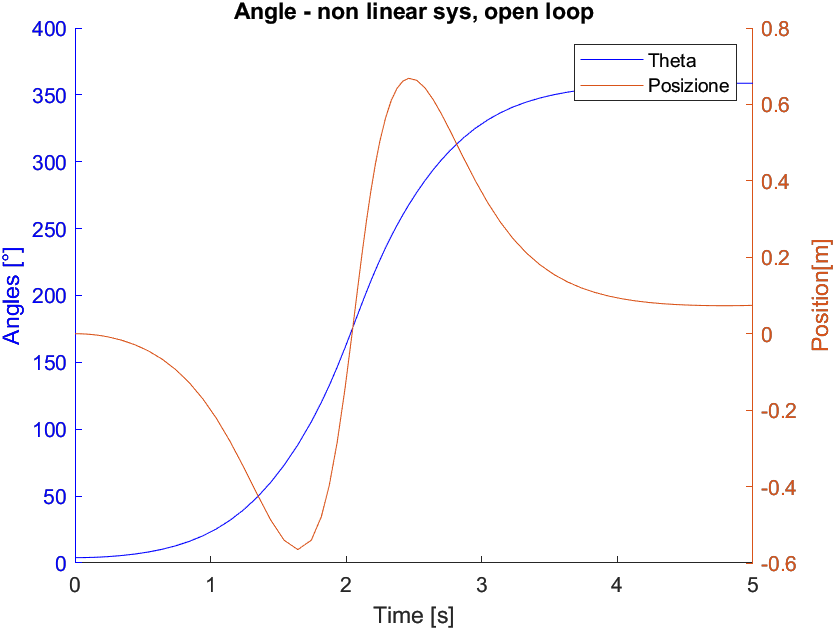
\includegraphics[width=0.6\textwidth]{Immagini/open_loop_response_non_linear.png}
	\caption{Risposta in anello aperto del sistema reale}
	\label{fig:open_loop_response_non_linear}
\end{figure}
La simulazione, il cui risultato è riportato in Fig.\ref{fig:open_loop_response_non_linear} è stata svolta per 5 secondi e con un angolo iniziale di 4°; il grafico mostra dunque l'andamento di $\theta$ nel tempo e della posizione che in termini matematici si esprime come $posizione = \phi \cdot{r_{ruota}}$
Si è inoltre creato un altro modello sfruttando il sistema lineare ottenuto prima  con l'obbiettivo di semplificare il problema e di velocizzare le simulazioni con lo scopo di testare rapidamente nuove tecniche di controllo che se avessero dato esito positivo sul modello lineare sarebbero poi state testate sul simulink che imita il comportamento reale del sistema.
\begin{figure}[H]
	\centering   	
	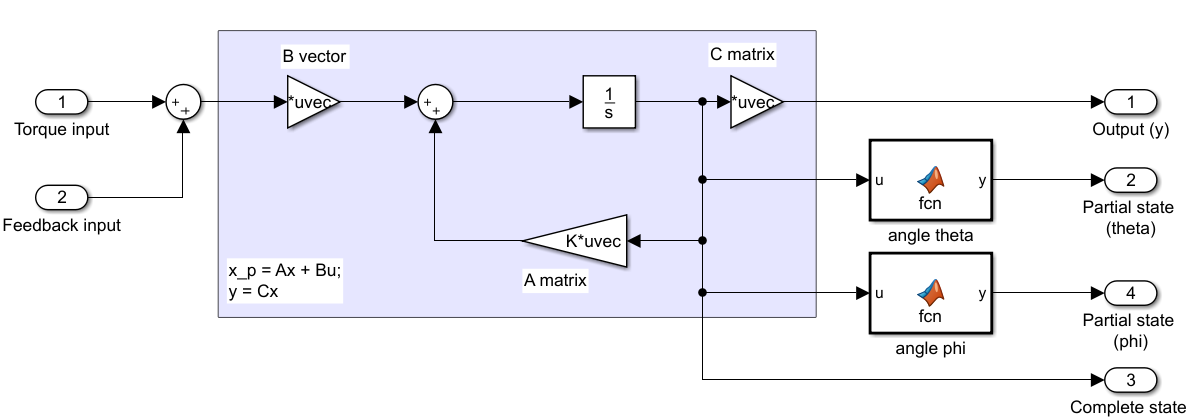
\includegraphics[width=1\textwidth]{Immagini/linear_system.png}
	\caption{Implementazione simulink del sistema linearizzato}
	\label{fig:linear_system}
\end{figure}

\begin{figure}[H]
	\centering   	
	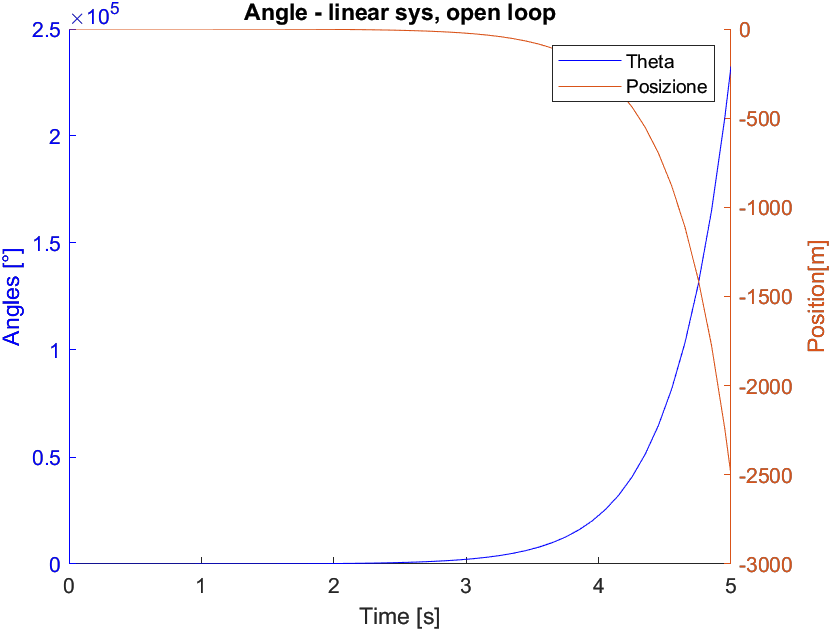
\includegraphics[width=0.6\textwidth]{Immagini/linear_open_loop.png}
	\caption{Risposta in anello aperto del sistema lineare}
	\label{fig:open_loop_response}
\end{figure}
In questo caso, la simulazione in anello aperto mostra che il sistema diverge; questo perché la linearizzazione ha senso attorno al punto di equilibrio da cui è stata ottenuta, distante da quel punto il sistema lineare non approssima più il sistema reale ed anche un eventuale controllo ottenuto da esso non garantisce buone performance distante da quel punto. Si nota, in Fig.\ref{fig:open_loop_response} che il punto di partenza è 4° e il sistema, lineare, diverga quasi immediatamente; la differenza con la risposta del sistema non lineare in Fig.\ref{fig:open_loop_response_non_linear}
\begin{figure}[H]
	\centering   	
	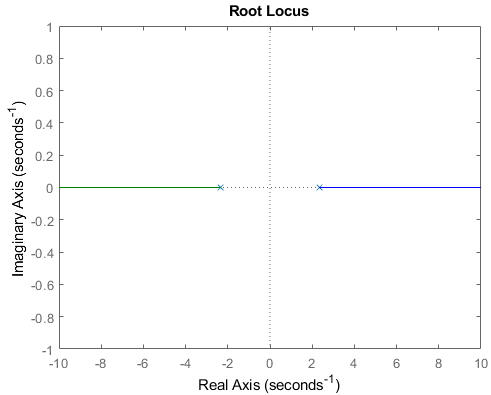
\includegraphics[width=0.6\textwidth]{Immagini/root_locus_open_loop.png}
	\caption{Posizione poli in anello aperto}
	\label{fig:open_loop_root}
\end{figure}
Come si vede in Fig.\ref{fig:open_loop_root}, ci sono due poli reali, uno negativo e uno positivo; questo dimostra come il sistema sia instabile in anello aperto e necessiti di controllo.


\section{Controllore}
Il problema della scelta del controllore è stato risolto mediante l'utilizzo dell'assegnazione degli autovalori ottenuti tramite retroazione dello stato; si affronta quindi un problema di regolazione: il moto del sistema è composto completamente dal moto libero che si vuole controllare e annullare in un tempo a piacere. Il posizionamento dei poli, e quindi la scelta del guadagno del regolatore, va eseguita sul solo sistema lineare:
\begin{figure}[H]
	\centering   	
	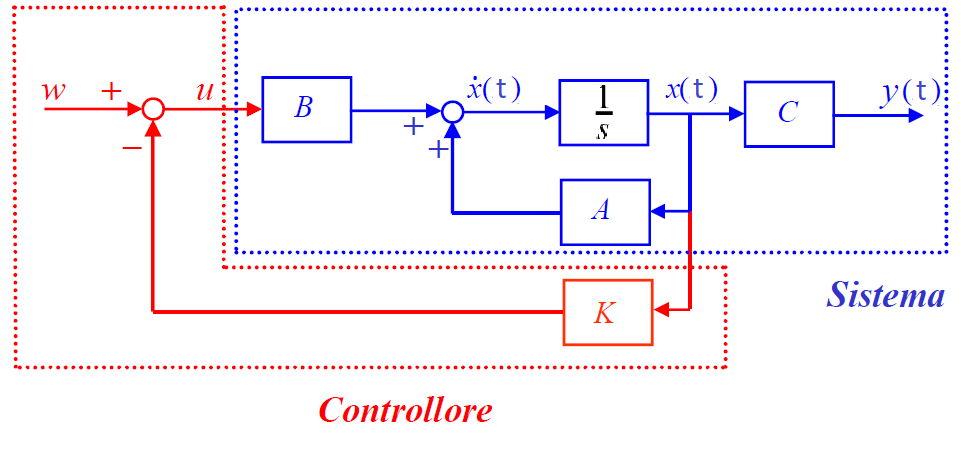
\includegraphics[width=0.70\textwidth]{Immagini/feedback_state.png}
	\caption{Schema concettuale del controllo,\cite{feedback_state}}
	\label{fig:feedback_state}
\end{figure}
Ciò che si nota in Fig.\ref{fig:feedback_state} può essere riscritto matematicamente:
\begin{center}
	$$
	\begin{cases}
	 \begin{array}{c}
		x\left(t\right)=Ax{\left(t\right)}+Bu\left(t\right)\\
		y{\left(t\right)}=Cx{\left(t\right)}+Du\left(t\right)
	\end{array}
	\end{cases}
	$$
	$$
	u{\left(t\right)}=-Kx{\left(t\right)}+w{\left(t\right)}	
	$$
\end{center}Dunque:
\begin{center}
	
	$$
	x{\left(t\right)}=Ax{\left(t\right)}+Bu{\left(t\right)}=Ax{\left(t\right)}+B{\left(-Kx{\left(t\right)}+w{\left(t\right)}\right)}
	$$
	$$
	=Ax{\left(t\right)}-BKx{\left(t\right)}+Bw\left(t\right)={\left(A-BK\right)}x{\left(t\right)}+Bw{\left(t\right)}
	$$
	$$
	A_{closedloop} =A-BK
	$$
\end{center}
Per scegliere il valore di guadagno del controllore, è necessario scegliere la posizione desiderata dei poli:
\begin{center}
	$$
	G{\left(S\right)}=\frac{\omega {\;}_n^{2\;} }{s^2 +2\xi \omega {\;}_n s+\omega {\;}_n^{2\;} }
	$$
\end{center}
\begin{center}
	in cui:
	$$
	\xi =0\ldotp 7
	$$
	$$
	\omega {\;}_{n\;} =2\bullet \pi \bullet f_{\mathrm{propria}}
	$$
\end{center}Dovendo posizionare due coppie di poli complessi coniugati si sono scelte due frequenze ad una decade di distanza
\begin{center}
	
	$$
	f_{\mathrm{propria\theta}} =  0.2
	$$
	$$
	f_{\mathrm{propria\phi}} =  0.02
	$$
\end{center}Per motivi esterni il motore ha una coppia massima molto limitata ed è stato dunque necessario posizionare i poli in modo che non fossero troppo veloci.
\begin{center}
	
	$$
	polo_{\theta} = \left(\begin{array}{c}
	-\frac{7\,\pi }{250}+\frac{\pi \,\sqrt{51}\,\mathrm{i}}{250}\\
	-\frac{7\,\pi }{250}-\frac{\pi \,\sqrt{51}\,\mathrm{i}}{250}
	\end{array}\right)
	$$
	$$
	polo_{\phi} = \left(\begin{array}{c}
	-\frac{7\,\pi }{25}+\frac{\pi \,\sqrt{51}\,\mathrm{i}}{25}\\
	-\frac{7\,\pi }{25}-\frac{\pi \,\sqrt{51}\,\mathrm{i}}{25}
	\end{array}\right)
	$$
\end{center}	Questi quattro poli si può notare che abbiano parte reale negativa; la stabilità in questo modo è raggiunta.\\
Con il comando \textit{place} di Matlab si ottine dunque:
\begin{center}

	$	K =[  -0.0023  , -0.0278, -28.1397  , -7.7022]$

\end{center}
Il sistema in anello chiuso ha i seguenti poli:
\begin{figure}[H]
	\centering   	
	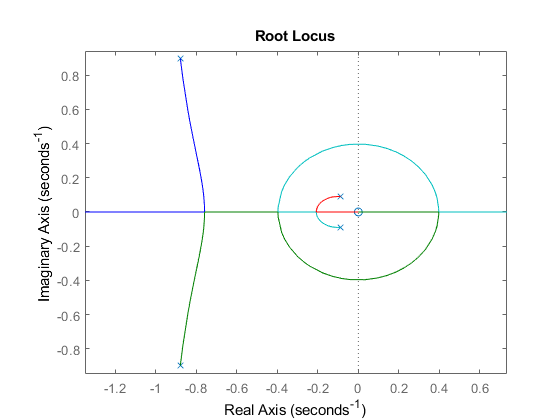
\includegraphics[width=1\textwidth]{Immagini/root_locus_closed_loop.png}
	\caption{Root locus del sistema in anello chiuso}
	\label{fig:closed_loop_root}
\end{figure}
Si va ora ad analizzare la risposta del sistema al controllo ottenuto nei punti precedenti, per assicurarci, che quanto scritto sopra valga oltre che nella teoria anche nella pratica:
\begin{figure}[H]
	\centering   	
	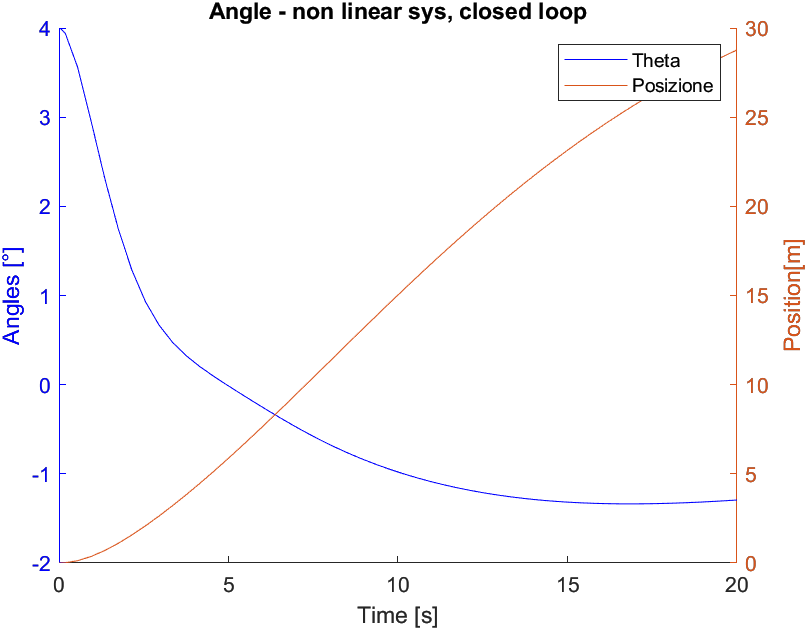
\includegraphics[width=0.7\textwidth]{Immagini/closed_loop_non_linear.png}
	\caption{Risposta del sistema non lineare in anello chiuso}
	\label{fig:closed_loop_non_linear_response}
\end{figure}
\begin{figure}[H]
	\centering   	
	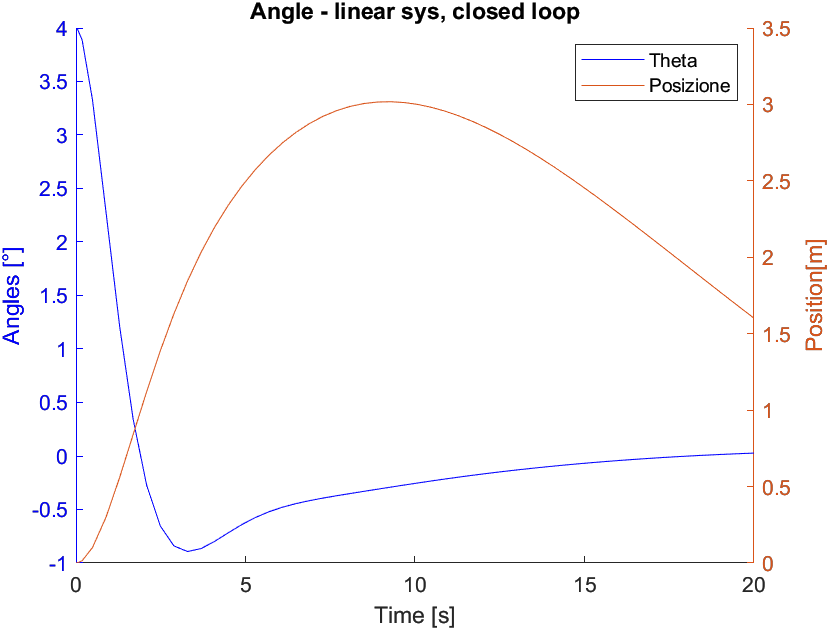
\includegraphics[width=0.7\textwidth]{Immagini/closed_loop_linear.png}
	\caption{Risposta del sistema lineare in anello chiuso}
	\label{fig:closed_loop_non_linear_response}
\end{figure}
TODO: come spieghiamo la differenza? rifare la simulazione?


\section{Motore}
Il passo successivo è stato quello di andare a modellizzare il motore presente a bordo dello Chassy; questo è necessario in quanto si deve tenere conto, in primo luogo, del ritardo che gli attuatori ( cioè il motore) introducono nel sistema e che per questo potrebbe diventare instabile.
\begin{figure}[H]
	\centering   	
	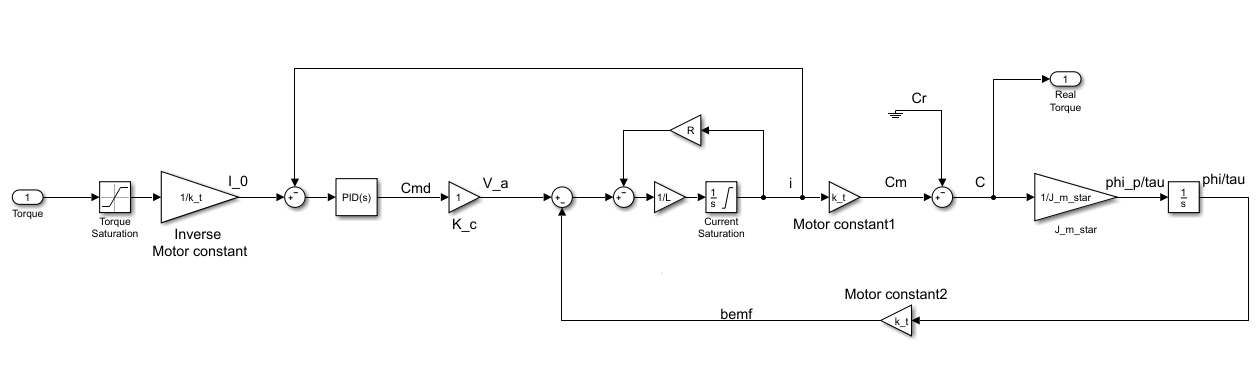
\includegraphics[width=1\textwidth]{Immagini/motor.png}
	\caption{Schema a blocchi del motore}
	\label{fig:motor}
\end{figure}

I valori delle componenti in Fig.\ref{fig:motor} sono presi dal datasheet del motore.
Il controllo del motore DC in questione e stato ottenuto tramite una retroazione in corrente che permette quindi di definire un setpoint alla corrente presente nel motore. Questo si è reso necessario poiché il controllore, attraverso il vettore K e lo stato del sistema, definisce la coppia che il motore dovrebbe erogare. In un motore DC la correlazione tra coppia erogata e corrente esiste ed è ben definita e si tratta di $k_t$ TODO equazione tra corrente e coppia\\
il controllore è stato così calcolato:

TODO anti wind up, uscita, grafici transitori, 
\begin{figure}[H]
	\centering   	
	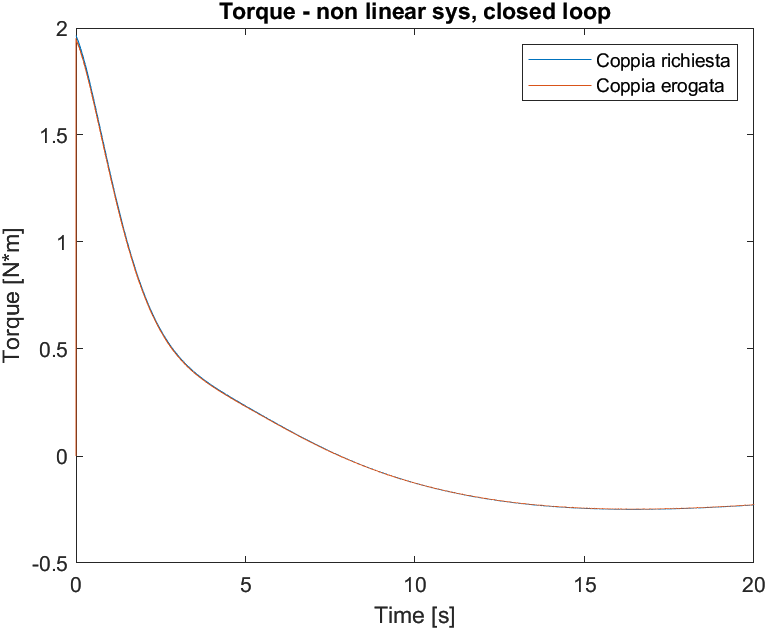
\includegraphics[width=0.7\textwidth]{Immagini/motore.png}
	\caption{Schema a blocchi del motore}
	\label{fig:motor}
\end{figure}
\begin{figure}[H]
	\centering   	
	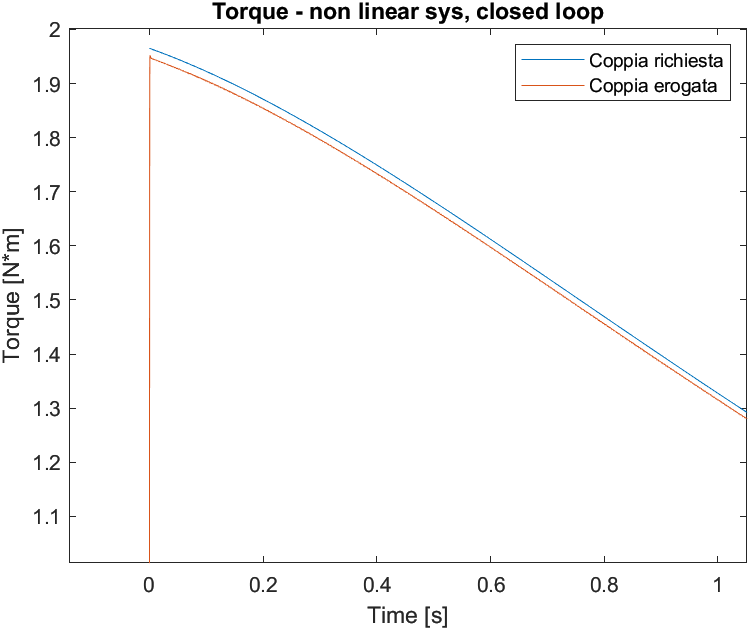
\includegraphics[width=0.7\textwidth]{Immagini/motore_zoom.png}
	\caption{Schema a blocchi del motore}
	\label{fig:motor}
\end{figure}